\documentclass[a4paper]{article}

\usepackage{amsmath}
\usepackage{tabularx}
\usepackage{todonotes}
%\usepackage{showframe}
\usepackage{tikz}
\newcommand{\specialcell}[2][c]{%
  \begin{tabular}[#1]{@{}c@{}}#2\end{tabular}}

\begin{document}
\section{Organization and Introduction}
\begin{itemize}
\item The Art of managing complexity
\begin{itemize}
\item Abstraction: Hiding details when they are not important
\item Discipline: Intentionally restricting your design choices to that you can work more productively at higher abstraction levels
\item The three -Y's
\begin{itemize}
\item Hierarchy: A system is divided into modules of smaller complexity
\item Modularity: Having well defined functions and interfaces
\item Regularity: Encouraging uniformity, so modules can be easily re-used
\end{itemize}
\end{itemize}
\item Bit: \textbf{B}inary dig\textbf{it}
\end{itemize}

\section{Binary Numbers}
\begin{itemize}
\item Powers of two:\\
\begin{tabular}{c|c|c}
$2^0= 1$ & $2^5=32$ & $2^{10}= 1024$\\ 
$2^1= 2$ & $2^6=64$ & $2^{11}= 2048$\\ 
$2^2= 4$ & $2^7=128$ & $2^{12}= 4096$\\ 
$2^3= 8$ & $2^8=256$ & $2^{13}= 8192$\\ 
$2^4= 16$ & $2^9=512$ & $2^{14}= 16384$\\ 
\end{tabular}
\item Binary to decimal conversion
\begin{align*}
10011_2&=2^4\times 1 +2^3\times 0 + 2^2\times 0 +2^1\times 1 +2^0\times 1\\
&=16 \times 1+8 \times 0+4 \times 0+2 \times 1+1 \times 1\\
&=16+0+0+2+1=19_{10}
\end{align*}
\item Convert decimal to binary (roughly). Example with $47_{10}$ to binary\\
\begin{tabular}{c|c|c|c|c}
$2^6=64$& is $64\leq 47$?&no&0&do nothing\\ 
$2^5=32$& is $32\leq 47$?&yes&1&47-32=15\\
$2^4=16$& is $16\leq 15$?&no&0&do nothing\\
$2^3=8$& is $8\leq 15$?&yes&1&15-8=7\\ 
$2^2=4$& is $4\leq 7$?&yes&1&7-4=3\\
$2^1=2$& is $2\leq 3$?&yes&1&3-2=1\\
$2^0=1$& is $1\leq 1$?&yes&1&1-1=0; done!\\
\end{tabular}\\
$\Rightarrow 47_{10}$ to binary is $0101111_2$ 
\item Binary values and range
\begin{itemize}
\item $N-$digit decimal number
\begin{itemize}
\item How many values: $10^N$
\item Range: $\lbrack 0,10^{N}-1\rbrack$
\item Example (3-digit number): $10^3=1000$ possible values, range:$\lbrack 0,999\rbrack$
\end{itemize}
\item $N-$bit binary number
\begin{itemize}
\item How many values: $2^N$
\item Range: $\lbrack 0,2^{N}-1\rbrack$
\item Example (3-digit number): $2^3=8$ possible values, range:$\lbrack 0,7\rbrack=\lbrack 000_2\text{ to }111_2\rbrack$
\end{itemize}
\end{itemize}
\item Hexadecimal (Base-16) Numbers\\
\begin{tabular}{c|c|c|c|c|c|c}
Decimal & Hexadecimal & Binary&{}&Decimal & Hexadecimal & Binary\\\hline
0&0&0000&{}&8&8&1000\\
1&1&0001&{}&9&9&1001\\
2&2&0010&{}&10&A&1010\\
3&3&0011&{}&11&B&1011\\
4&4&0100&{}&12&C&1100\\
5&5&0101&{}&13&D&1101\\
6&6&0110&{}&14&E&1110\\
7&7&0111&{}&15&F&1111\\
\end{tabular}
\item Bits, Bytes, Nibbles...
\[\begin{array}{*{20}{c}}
{\underbrace 1_{{\text{MSB}}}001011\underbrace 0_{{\text{LSB}}}}&{\overbrace {1001\underbrace {0110}_{{\text{nibble}}}}^{{\text{Byte}}}}&{\underbrace {{\text{CE}}}_{{\text{MSB}}}{\text{BF9A}}\underbrace {{\text{D7}}}_{{\text{LSB}}}}
\end{array}\]
Where MSB=Most significant Bit and LSB=Least significant Bit
\item Addition in base two works exactly the same as in base 10, using carries
\item Overflow
\begin{itemize}
\item Digital systems operate on a fixed number of bits
\item Addition overflows when the result is too big to fit in the available number of bits
\end{itemize}
\item Signed Binary Numbers
\begin{itemize}
\item Sign/Magnitude Numbers
\begin{itemize}
\item 1 sign bit, $N-1$ magnitude bits
\item Sign bit is the most significant (left-most) bit
\item Example: 4-bit sign/mag repr. of $\pm 6$:
\begin{itemize}
\item $+6=\textbf{0}110$
\item $-6=\textbf{1}110$
\end{itemize}
\item Range of an $N-$bit sign/magnitude number:\\
$\lbrack -\left( 2^{N-1}-1\right),2^{N-1}-1\rbrack$
\item Problems:
\begin{itemize}
\item Addition doesn't work
\item Two representations of 0 ($\pm 0$): 1000 and 0000
\item Introduces complexity in the processor design
\end{itemize}
\end{itemize}
\item One's Complement Numbers
\begin{itemize}
\item A negative number is formed by reversing the bits of the positive number (MSB still indicates the sign of the integer)\\
\begin{tabular}{|c|c|c|c|c|c|c|c|c|c|c|}
\hline
$2^7$&$2^6$&$2^5$&$2^4$&$2^3$&$2^2$&$2^1$&$2^0$&{}&One's Compl.&Unsigned\\\hline\hline
0&0&0&0&0&0&0&0&$=$&0&0\\
0&0&0&0&0&0&0&1&$=$&1&1\\
0&0&0&0&0&0&1&0&$=$&2&2\\
\dots&\dots&\dots&\dots&\dots&\dots&\dots&\dots&\dots&\dots&\dots\\
0&1&1&1&1&1&1&1&$=$&127&127\\
1&0&0&0&0&0&0&0&$=$&-127&128\\
1&0&0&0&0&0&0&1&$=$&-126&129\\
\dots&\dots&\dots&\dots&\dots&\dots&\dots&\dots&\dots&\dots&\dots\\
1&1&1&1&1&1&0&1&$=$&-2&253\\
1&1&1&1&1&1&1&0&$=$&-1&254\\
1&1&1&1&1&1&1&1&$=$&-0&255\\\hline
\end{tabular}
\item Range of $n-$bit number: $\lbrack -2^{n-1}-1,2^{n-1}-1\rbrack$, 8 bits:$\lbrack -127,127\rbrack$
\item Addition: Done using binary addition with end-around carry. If there is a carry out of the MSB of the sum, this bit must be added to the LSB of the sum
\end{itemize}
\item Two's Complement Numbers
\begin{itemize}
\item Don't have same problems as sign/magnitude numbers:
\begin{itemize}
\item addition works
\item Single representation for 0
\end{itemize}
\item Has advantages over one's complement:
\begin{itemize}
\item Has a single 0 representation
\item Eliminates the end-around carry operation required in one's complement addition.
\end{itemize}

\item A negative number is formed by reversing the bits of the positive number (MSB still indicates the sign of the integer) and adding 1:\\
\begin{tabular}{|c|c|c|c|c|c|c|c|c|c|c|}
\hline
$2^7$&$2^6$&$2^5$&$2^4$&$2^3$&$2^2$&$2^1$&$2^0$&{}&Two's Compl.&Unsigned\\\hline\hline
0&0&0&0&0&0&0&0&$=$&0&0\\
0&0&0&0&0&0&0&1&$=$&1&1\\
0&0&0&0&0&0&1&0&$=$&2&2\\
\dots&\dots&\dots&\dots&\dots&\dots&\dots&\dots&\dots&\dots&\dots\\
0&1&1&1&1&1&1&1&$=$&127&127\\
1&0&0&0&0&0&0&0&$=$&-128&128\\
1&0&0&0&0&0&0&1&$=$&-127&129\\
\dots&\dots&\dots&\dots&\dots&\dots&\dots&\dots&\dots&\dots&\dots\\
1&1&1&1&1&1&0&1&$=$&-3&253\\
1&1&1&1&1&1&1&0&$=$&-2&254\\
1&1&1&1&1&1&1&1&$=$&-1&255\\\hline
\end{tabular}
\item Same as unsigned binary, but the most significant bit (MSB) has value of $-2^{N-1}$
\begin{itemize}
\item Most positive 4-bit number: 0111
\item Most negative 4-bit number: 1000
\end{itemize}
\item The most significant bit still indicates the sign (1=neg., 0=pos.)
\item Range of an $N-$bit two's comp. number: $\lbrack -2^{N-1},2^{N-1}-1\rbrack$, 8 bits:$\lbrack -128,127\rbrack$
\end{itemize}
\end{itemize}
\item Increasing bit width (assume from $N$ to $M$, with $M>N$): 
\begin{itemize}
\item Sign-extension
\begin{itemize}
\item Sign bit is copied into MSB
\item Number value remains the same
\item Give correct result for two's compl. numbers
\item Example 1:
\begin{itemize}
\item 4-bit representation of $3=\textbf{0}011$
\item 8-bit sign-extended value: $\textbf{00000}011$
\end{itemize}
\item Example 2:
\begin{itemize}
\item 4-bit representation of $-5=\textbf{1}011$
\item 8-bit sign-extended value: $\textbf{11111}011$
\end{itemize}
\end{itemize}
\item Zero-extension
\begin{itemize}
\item Zeros are copied into MSB
\item Value will change for negative numbers
\item Example 1:
\begin{itemize}
\item 4-bit value: $0011_2=3_{10}$
\item 8-bit zero-extended value: $\textbf{0000}0011_2=3_{10}$
\end{itemize}
\item Example 2:
\begin{itemize}
\item 4-bit value: $1011_2=-5_{10}$
\item 8-bit zero-extended value: $\textbf{0000}1011_2=\textbf{$11_{\textbf{10}}$}$
\end{itemize}
\end{itemize}
\end{itemize}
\end{itemize}

\section{Short Introduction to Electrical Engineering (EE Perspective)}
\begin{itemize}
\item The goal of circuit design is to optimize:
\begin{itemize}
\item Area: Net circuit area is proportional to the cost of the device
\item Speed/Throughput: We want circuits that work  faster, or do more
\item Power/Energy
\begin{itemize}
\item Mobile devices need to work with a limited power supply
\item High performance devices dissipate more than 100W/$cm^2$
\end{itemize}
\item Design time
\begin{itemize}
\item Designers are expensive
\item The competition will not wait for you
\end{itemize}
\end{itemize}
\item (Frank's) Principles for engineering
\begin{itemize}
\item Good engineers are lazy: They do not want to work unnecessarily, be creative
\item They know how to ask the question ``why''?: take nothing for granted
\item Engineering is not a religion: Use what works best for you
\item Keep it simple and stupid: Engineers' job is to manage complexity
\end{itemize}
\item Building blocks for microchips
\begin{itemize}
\item Conductors: Metals (Aluminium, Copper)
\item Insulators: Glass (SiO$_2$), Air
\item Semiconductors: Silicon (Si), Germanium (Ge)
\end{itemize}
\item N-type Doping: Add extra electron (negatively charged), zone becomes negatively charged\todo{Maybe add a definition or a better explanation}
\item P-type Doping: Remove electron, zone becomes positively charged
\item Semiconductors:
\begin{itemize}
\item You can ``Engineer'' its properties, i.e.
\begin{itemize}
\item Make it P type by injecting type-III elements (b, Ga, In)
\item Make it N type by injecting elements from type-V (P, As)
\end{itemize}
\item You can combine P and N regions to each other, from a pure semiconductor
\item Allows you to make interesting electrical devices (Diodes, Transistors, Thrystors)
\end{itemize}
\item pMOS is a P type transistor, nMOS an N type transistors; combined they are a CMOS
\item CMOS (Properties)
\begin{itemize}
\item No input current: Capacitive input, no resistive path from the input
\item No current when output is at logic levels: Little static power, current is needed only when switching
\item Electrical properties determined directly by geometry: A transistor that is 2 times larger drives twice the current
\item Very simple to manufacture: pMOS and nMOS can be manufactures on the same substrate
\end{itemize}
\item CMOS Gate Structure
\begin{itemize}
\item The general form used to construct any inverting logic, such as: NOT, NAND, NOR
\begin{itemize}
\item The networks may consist of transistors in series or parallel
\item When transistors are in parallel, the network is ON if either transistor is ON
\item When transistors are in series, the network is ON only if all transistors are ON
\end{itemize}
\item In a proper logic gate: One of the networks should be ON and the other OFF at any given time
\item Use the rule of conduction complements:
\begin{itemize}
\item When nMOS transistors are in series, the pMOS transistor must be in parallel
\item When nMOS transistors are in parallel, the pMOS transistors must be in series
\end{itemize}
\end{itemize}
\todo[inline]{Add picture on slide 34, 03 - EEPerspective}
\item Logic Gates
\begin{itemize}
\item Perform logic functions: Inversion (NOT), AND, OR, NAND, NOR, etc.
\item Single input: NOT gate, buffer
\item Two-input: AND, OR, XOR, NAND, NOR, XNOR\\
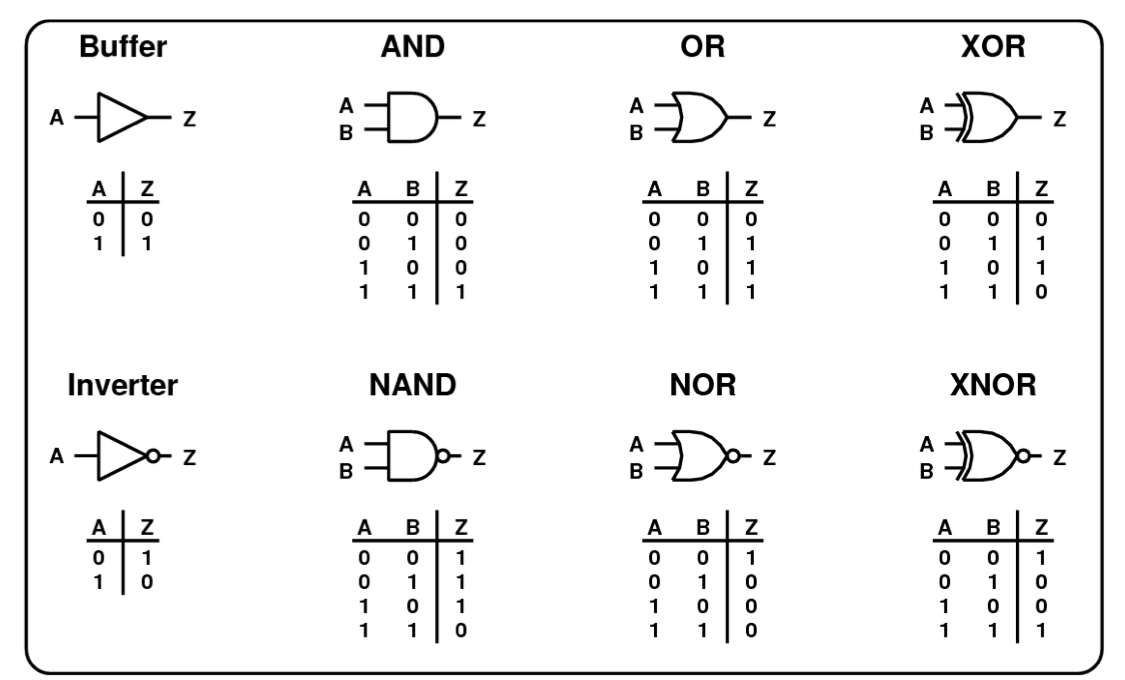
\includegraphics[scale=0.27]{Figures/commonLogicGates.jpg}
\item Multiple-Input:
\begin{itemize}
\item 3, 4, or even more input AND, OR, XOR gates
\item Compound gates
\begin{itemize}
\item AND-OR
\item OR-AND
\item AND-OR-INVERT
\item OR-AND-INVERT
\end{itemize}
\item Other cells: Multiplexers and Adders
\end{itemize}
\end{itemize}
\item Logic Levels
\begin{itemize}
\item Define ranges of discrete voltages to represent 1 and 0 (i.e. 0 for ground and 1 for 5V ($V_{DD}$)) and allow for noise.
\end{itemize}
\item Noise: Is anything that degrades the signal (i.e. resistance, power supply noise, etc.)
\item Moore's Law
\begin{itemize}
\item \emph{``Number of transistors that can be manufactured doubles roughly every 18 months.''} - Gordon Moore, 1965
\end{itemize}
\item How do we keep Moore's Law:
\begin{itemize}
\item Manufacturing smaller structures: some structures are already a few atoms in size
\item Developing materials with better properties
\item Optimizing the manufacturing steps
\item New technologies
\end{itemize}
\item Power consumption
\begin{itemize}
\item Power = Energy consumed per unit time
\item Two types of power consumption:
\begin{enumerate}
\item Dynamic power consumption: Power to charge transistor gate capacitances \[P_{\text{dynamic}}=\frac{1}{2}CV_{DD}^2f\]
\item Static power consumption: Power consumed when no gates are switching, caused by the leakage current \[P_{\text{static}}=I_{DD}V_{DD}\]
\end{enumerate}
\end{itemize}
\end{itemize}

\section{Combinational Circuits: Theory}
\begin{itemize}
\item Circuit elements. A circuit consists of:
\begin{itemize}
\item Inputs
\item Outputs
\item Nodes (wires): Connections between I/O and circuit elements. To count them, look at
\begin{itemize}
\item Outputs of every circuit elements
\item Inputs to the entire circuit
\end{itemize}
\item Circuit elements
\end{itemize}
\item Types of Logic Circuits
\begin{itemize}
\item Combinational Logic
\begin{itemize}
\item Memoryless
\item Outputs determined by current values of inputs
\item In some books called Combinatorial Logic
\end{itemize}
\item Sequential Logic
\begin{itemize}
\item Has Memory
\item Outputs determined by previous and current values of inputs
\end{itemize}
\end{itemize}
\item Rules of Combinational Composition
\begin{itemize}
\item Every circuit element is itself combinational
\item Every node of the circuit is either
\begin{itemize}
\item Designated as an input to the circuit
\item Connects to exactly one output terminal of a circuit element
\end{itemize}
\item The circuit contains no cyclic paths: Every path through the circuit visits each node at most once

\end{itemize}
\item Boolean Equations\footnote{For a more in depth look, use the material from Diskrete Mathematik}
\begin{itemize}
\item Functional specifications of outputs in terms of inputs.
\end{itemize}
\item Boolean Algebra
\begin{itemize}
\item Set of axioms and theorems to simplify Boolean equations
\item Like regular algebra, but in some cases simpler because variables only have 1 or 0 as a value
\item Axioms and theorems obey the principles of duality:
\begin{itemize}
\item Stay corrected if: ANDs and ORs interchanged and 0's and 1's interchanged
\item Example:\\
\begin{tabular}{l|l}
{}&Dual\\\hline
$\overline{0}=1$&$\overline{1}=0$\\
$B\cdot\overline{B}=0$&$B+\overline{B}=1$
\end{tabular}

\end{itemize}
\end{itemize}
\item Boolean Axioms\\
\begin{tabular}{|l|l|l|l|l|}\hline
{}&Axiom&{}&Dual&Name\\\hline
$A1$ & $B=0$ if $B\not = 1$ & $A1'$ & $B=1$ if $B\not=0$ & Binary Field\\
$A2$ & $\overline{0}=1$ & $A2'$ & $\overline{1}=0$ & NOT  \\
$A3$ & $0\cdot 0=0$ & $A3'$ & $1+1=1$ & AND/OR     \\
$A4$ & $1\cdot 1=1$ & $A4'$ & $0+0=0$ & AND/OR    \\
$A5$ & $0\cdot 1=1\cdot 0=0$ & $A5'$ & $1+0=0+1=1$ & AND/OR \\ \hline
\end{tabular}
\\Duality: If the symbols 0 and 1 and the operators $\cdot$ (AND) and $+$ (OR) are interchanged, the statement will still be correct
\item Boolean Theorems\\
\resizebox{13cm}{!}{
\begin{tabular}{|l|l|l|l|l|}\hline
{}&Theorem&{}&Dual&Name\\\hline\hline
$T1$ & $B\cdot 1=B$ & $T1'$ & $B+0=B$ & Identity\\\hline
$T2$ & $B\cdot 0=0$ & $T2'$ & $\overline{1}=0$ & Null Element  \\\hline
$T3$ & $B\cdot B=B$ & $T3'$ & $1+1=1$ & Idempotency     \\\hline
$T4$ & {} & $\overline{\overline{B}}=B$ & {} & Involution    \\\hline
$T5$ & $B\cdot\overline{B}=0$ & $T5'$ & $1+0=0+1=1$ & Complements \\ \hline
$T6$ & $B\cdot C=C\cdot B$ & $T6'$ & $B+C=C+B$ & Commutativity	\\\hline
$T7$ & $(B\cdot C)\cdot D= B\cdot (C\cdot D)$ & $T7'$ & $(B+C)+D = B+(C+D)$ & Associtivity	\\\hline
$T8$ & $(B\cdot C)+(B\cdot D)=B\cdot (C+D)$ & $T8'$ & $(B+C)\cdot (B+D)=B+(C\cdot D)$ & Distributivity	\\\hline
$T9$ & $B\cdot (B+C)=B$ & $T9'$ & $B+(B\cdot C)=B$ & Covering	\\\hline
$T10$ & $(B\cdot C) + (B\cdot \overline{C})=B$ &$T10'$& $(B+C)\cdot (B+\overline{C})=B$& Combining\\\hline
$T11$ &\specialcell{$(B\cdot C)+(\overline{B}\cdot D)+(C\cdot D)$\\$=B\cdot C+\overline{B}\cdot D$} & $T11'$ & \specialcell{$(B+t C)\cdot(\overline{B}+ D)\cdot(C+ D)$\\$=(B + C)\cdot(\overline{B}+ D)$}  & Consensus	\\\hline
$T12$ & $\overline{B_0\cdot B_1\cdot B_2\cdot\dots}= (\overline{B_0}+\overline{B_1}+\overline{B_2}+\dots)$ & $T12'$ & $\overline{B_0 +  B_1+ B_2+\dots}= (\overline{B_0}\cdot\overline{B_1}\cdot\overline{B_2}\cdot\dots)$ & \specialcell{De Morgan's\\ Theorem}\\
\hline
\end{tabular}
}

\item Bubble Pushing
\begin{itemize}
\item Pushing bubbles backward (from the output) or forward (from the inputs) changes the body of the gate from AND to OR or vice versa
\begin{itemize}
\item Pushing a bubble from the output back to the inputs puts bubbles on all gate inputs
\item Pushing bubbles on all gate inputs forward toward the output puts a bubble on the output and changes the gate body
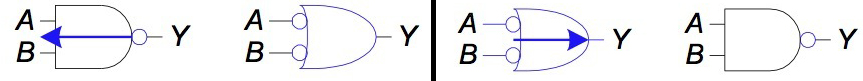
\includegraphics[scale=0.35]{Figures/bubblePushing.jpg}
\end{itemize}
\item Rules:
\begin{itemize}
\item Begin at the output of the circuit and work toward the inputs
\item Push any bubbles on the final output back toward the inputs
\item Draw each gate in a form so that bubbles cancel
\end{itemize}
\end{itemize}
\end{itemize}

\section{Combinational Circuits Design}
\begin{itemize}
\item Some Definitions:
\begin{itemize}
\item Complement: variable with a bar over it ($\overline{A},\overline{B},\overline{C}$)
\item Literal: variable or its complement ($A,\overline{A},B,\overline{B},C,\overline{C}$)
\item Implicant: product (AND) of literals ($A\cdot B\cdot \overline{C}$)
\item Minterm: product (AND) that includes all input variables ($A\cdot B \cdot \overline{C}$)
\item Maxterm: sum (OR) that includes all input variables ($A+\overline{B}+\overline{C}$)
\end{itemize}
\item Sum-of-Products (SOP) Form
\begin{itemize}
\item All boolean equations can be written in SOP form
\begin{itemize}
\item Each row in a truth table has a minterm
\item A minterm is a product (AND) of literals
\item Each minterm is TRUE for that row (and only that row)
\end{itemize}
\item Formed by ORing the minterms for which the output is TRUE
\end{itemize}
\item The Dual: Product-of-Sums (POS) Form
\begin{itemize}
\item Al Boolean equations can be written in POS form
\begin{itemize}
\item Each row in a truth table has a maxterm
\item A minterm is a sum (OR) of literals
\item Each minterm is FALSE for that row (and only that row)
\end{itemize}
\item Formed by ANDing the maxterms for which the output is FALSE
\end{itemize}
\item Karnaugh Maps (K-Maps)
\begin{itemize}
\item Boolean expressions can be minimized by combining terms
\item K-maps minimize equations graphically
\item Rules:
\begin{itemize}
\item Special order for bit combinations: $\mathop {00,01,11,10}\limits^{
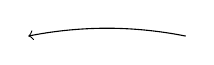
\begin{tikzpicture}
\draw[<-] (0,0) parabola bend (1,0.1) (2,0);
\end{tikzpicture}
}$ (only one bit changes to the next)
\item Every 1 in a K-map must be circled at least once
\item Each circle must span a power of 2 ($2^0$ included) squares in each direction 
\item Each circle must be as large as possible
\item A circle may wrap around the edges of the K-map
\item A ``Don't care'' $(X)$ is circled only if it helps minimize the equation
\end{itemize}
\end{itemize}
\item Circuit schematics 
\begin{itemize}
\item Inputs: left (or top) side of a schematic
\item Outputs: right (or bottom) side of a schematic
\item Circuits should flow from left to right
\item Straight wires are better than wires with multiple corners
\item Wires always connect at a T junction
\item A dot where wires cross indicated a connection between the wires
\item Wires crossing without a dot make no connection
\end{itemize}
\item Additional Logic Levels: $X$ and $Z$
\begin{itemize}
\item Contention: $X$
\begin{itemize}
\item When a signal is being driven to 1 and 0 simultaneously
\item Not a real level, could be any value (1,0 or something in between)
\item Usually a problem:
\begin{itemize}
\item Two outputs drive one node to opposite values
\item Normally there should only be one driver for every connection
\end{itemize}
\item WARNING: ``Don't care'' and ``contention'' are both called $X$
\begin{itemize}
\item These are not the same
\item Verilog uses $X$ for both, VHDL uses ``-'' for don't care, and ``$X$'' for contention
\item Don't care: degree of freedom that is fixed at implementation time
\item Contention: a bug really, undetermined behaviour
\end{itemize}
\end{itemize}
\item High-impedance or tri-state (or Floating): $Z$
\begin{itemize}
\item When an output is not driving to any specific value
\item Means the output is disconnected
\item Not a real level, some other output is able to determine the level
\item Output is called Floating, high impedance, tri-stated, or high-$Z$
\item Floating output might be 0, 1 or somewhere in between
\item Floating nodes are used in tri-state busses:
\begin{itemize}
\item Many different drivers share one common connection
\item Exactly one driver is active at any time
\item All the other drivers are ``disconnected''
\item The disconnected drivers are said to be floating, allowing exactly one node to drive
\item More than one input can listen to the shared bus without problems
\end{itemize}
\end{itemize}
\end{itemize}
\item Combinational Building Blocks
\begin{itemize}
\item Combinational logic is often grouped into larger building blocks to build more complex systems
\item Hide the unnecessary gate-level details to emphasize the function of the building block (full adders, priority circuits, etc.)
\end{itemize}
\item Multiplexer (Mux)
\begin{itemize}
\item Selects between one of $N$ inputs to connect to the output
\item Needs $\log_2N-$bit control input
\item A 4:1 Multiplexer can be implemented with:
\begin{itemize}
\item Two-level logic
\item Tristate buffers
\item Tree of 2:1 muxes
\end{itemize}
\item In general, a $2^N-$input multiplexer can be programmed to perform any $N-$input logic function by applying 0's and 1's to the appropriate data inputs
\end{itemize}
\item Decoders
\begin{itemize}
\item $N$ inputs, $2^N$ outputs
\item One-hot outputs: only one output HIGH at once
\end{itemize}
\item Timing
\begin{itemize}
\item Propagation delay: $t_{pd}=$ max delay from input to output
\item Contamination delay: $t_{cd}=$ min delay from input to output\\
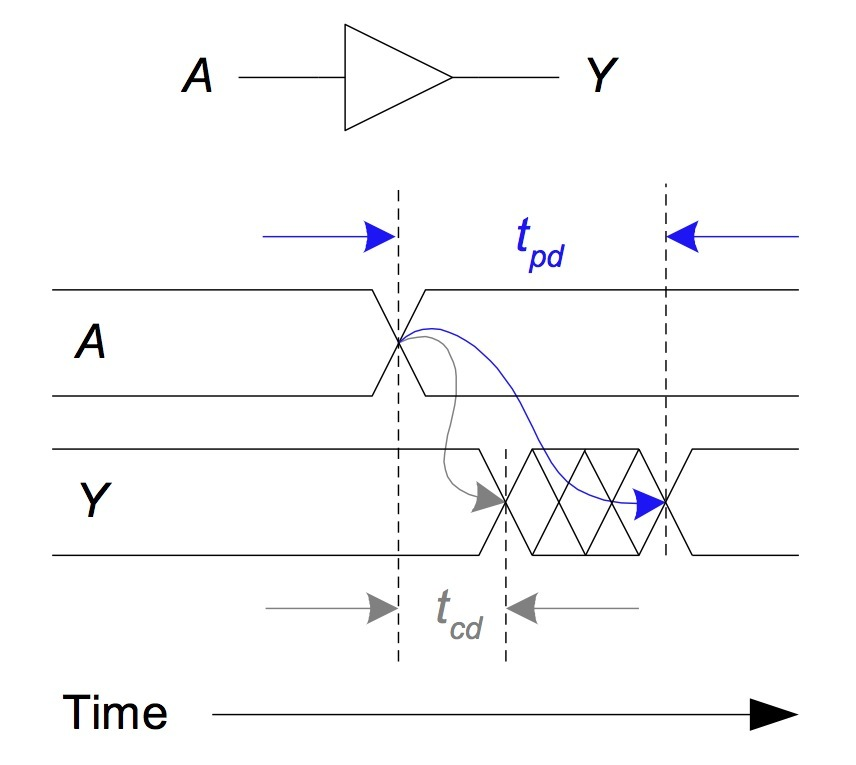
\includegraphics[scale=0.3]{Figures/PropContDelay.jpg}
\item Delay is caused by 
\begin{itemize}
\item capacitance and resistance in a circuit
\item Speed of light limitation (not as fast as you think)
\end{itemize}
\item Reasons why $t_{pd}$ and $t_{cd}$ may be different:
\begin{itemize}
\item Different rising and falling delays
\item Multiple inputs and outputs, some of which are faster than other
\item Circuits slow down when hot and speed up when cold
\end{itemize}
\item Critical (Long) and short paths\\
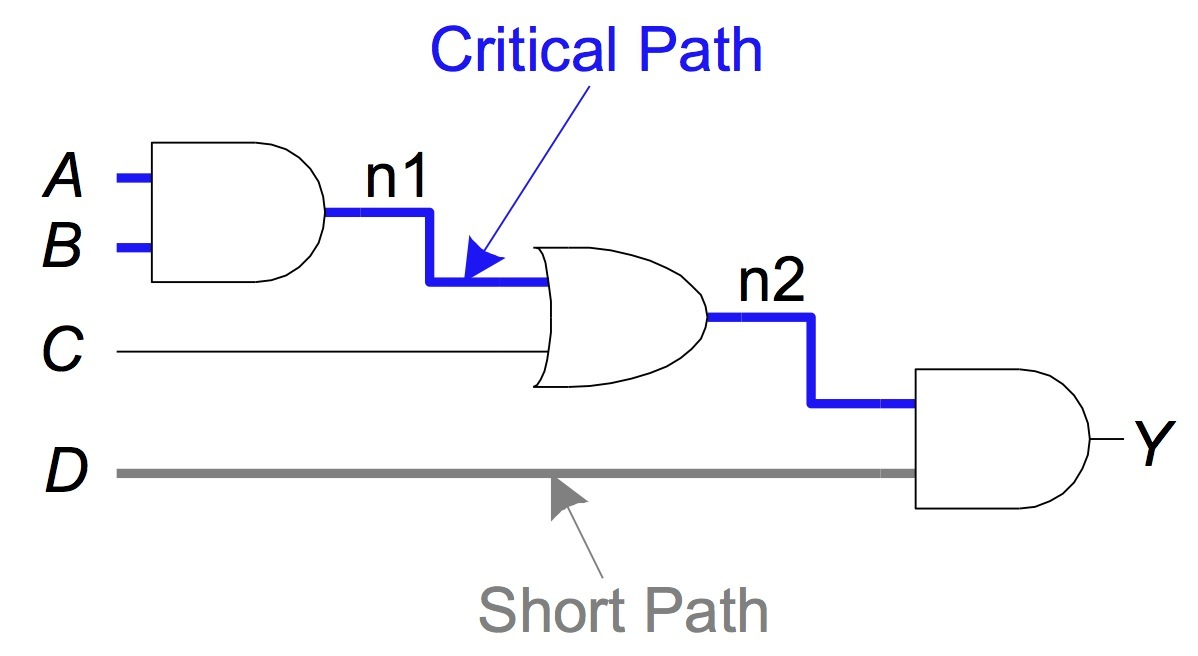
\includegraphics[scale=0.25]{Figures/CriticalAndShortPath.jpg}
\begin{itemize}
\item Critical (Long) path: $t_{pd}=2t_{pd\_\text{AND}}+t_{pd\_\text{OR}}$
\item Short path: $t_{cd}=t_{cd\_\text{AND}}$
\end{itemize}
\item Propagation Times\\
\begin{tabular}{l|l}
Gate & $t_{pd}$(ps)\\\hline
NOT & 30\\
$2-$input AND & 60\\
$3-$input AND & 80\\
$4-$input OR & 90\\
tristate ($A$ to $Y$) & 50\\
tristate (enable to $Y$) & 35
\end{tabular}
\end{itemize}
\item Glitches
\begin{itemize}
\item Glitch: when a single input change causes multiple output changes
\item Glitches don't cause problems because of synchronous design conventions
\item But it's important to recognize a glitch when you see one in timing diagrams
\item In general a glitch can occur when a change in a single variable crosses the boundary between two prime implicants in a $K-$map.
\item You \textbf{can't} get rid of all glitches - simultaneous transitions on multiple inputs can also cause glitches
\end{itemize}
\end{itemize}

\section{Field Programmable Gate Array (FPGA)}
\begin{itemize}
\item Logic arrays
\begin{itemize}
\item Programmable logic arrays (PLAs)
\begin{itemize}
\item AND array followed by OR array
\item Perform combinational logic only
\item Fixed internal connections
\item Composed of:
\begin{itemize}
\item LUTs (LookUp Tables): perform combinational logic
\item Flip-flops: perform sequential functions
\item Multiplexers connect LUTs and flip-flops
\end{itemize}
\end{itemize}
\item Field programmable gate arrays (FPGAs)
\begin{itemize}
\item Array of configurable logic blocks (CLBs)
\item Perform combinational and sequential logic
\item Programmable internal connections
\item Composed of:
\begin{itemize}
\item CLBs (Configurable Logic Blocks): Perform logic
\item IOBs (Input/Output Buffers): Interface with outside world
\item Programmable interconnection: connect CLBs and IOBs
\end{itemize}
\item Some FPGAs include other building blocks such as multipliers and RAMs
\end{itemize}
\end{itemize}
\end{itemize}


\end{document}